\newcommand{\half}{$\frac{1}{2}$}

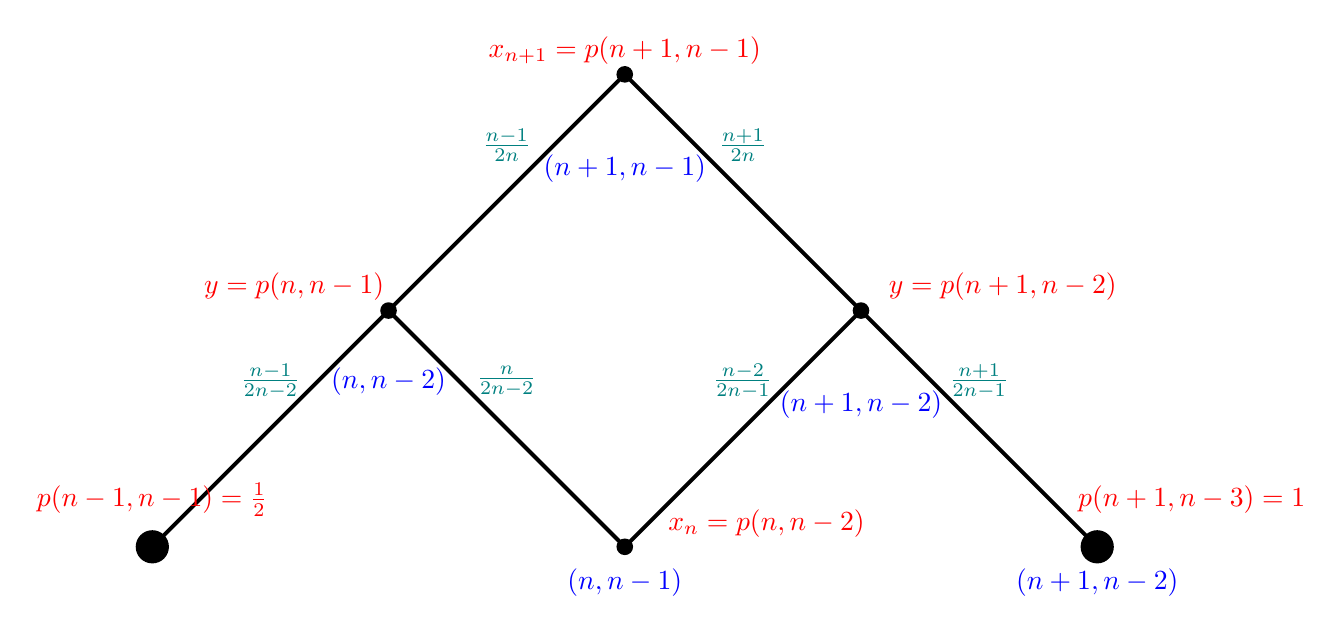
\begin{tikzpicture}[line cap=round,line join=round,x=3cm,y=3cm]

\draw[line width=0.5mm] ( 1,1) -- ( 0,0) node[sloped, pos=0.5, allow upside down]{\arrowIn}; 
\draw[line width=0.5mm] (-1,1) -- ( 0,0) node[sloped, pos=0.5, allow upside down]{\arrowIn}; 
\draw[line width=0.5mm] ( 0,2) -- ( 1,1) node[sloped, pos=0.5, allow upside down]{\arrowIn}; 
\draw[line width=0.5mm] ( 0,2) -- (-1,1) node[sloped, pos=0.5, allow upside down]{\arrowIn}; 
\draw[line width=0.5mm] ( 1,1) -- ( 2,0) node[sloped, pos=0.5, allow upside down]{\arrowIn}; 
\draw[line width=0.5mm] (-1,1) -- (-2,0) node[sloped, pos=0.5, allow upside down]{\arrowIn}; 

\fill ( 0,0) circle[radius=3pt];
\fill (-1,1) circle[radius=3pt];
\fill ( 1,1) circle[radius=3pt];
\fill ( 0,2) circle[radius=3pt];
\fill ( 2,0) circle[radius=6pt];
\fill (-2,0) circle[radius=6pt];


\node[text=red ] at ( 0.6 , 0.1) {$x_{n}=p(n,n-2)$};
\node[text=red ] at (-1.4 , 1.1) {$y=p(n,n-1)$};
\node[text=red ] at ( 0   , 2.1) {$x_{n+1}=p(n+1,n-1)$};
\node[text=red ] at ( 1.6 , 1.1) {$y=p(n+1,n-2)$};
\node[text=red ] at ( 2.4 , 0.2) {$p(n+1,n-3)=1$};
\node[text=red ] at (-2   , 0.2) {$p(n-1,n-1)=\frac{1}{2}$};

\node[text=blue] at ( 0  , -0.15) {$(n,n-1)$};
\node[text=blue] at ( 2  , -0.15) {$(n+1,n-2)$};
\node[text=blue] at ( 0  ,  1.6 ) {$(n+1,n-1)$};
\node[text=blue] at (-1 ,   0.7 ) {$(n,n-2)$};
\node[text=blue] at ( 1 ,   0.6 ) {$(n+1,n-2)$};

\node[text=teal] at (-0.5 , 1.7) {$\frac{n-1}{2n}$};
\node[text=teal] at ( 0.5 , 1.7) {$\frac{n+1}{2n}$};
\node[text=teal] at (-0.5 , 0.7) {$\frac{n}{2n-2}$};
\node[text=teal] at ( 0.5 , 0.7) {$\frac{n-2}{2n-1}$};
\node[text=teal] at ( 1.5 , 0.7) {$\frac{n+1}{2n-1}$};
\node[text=teal] at (-1.5 , 0.7) {$\frac{n-1}{2n-2}$};


\end{tikzpicture}

